\documentclass[10pt]{beamer}
\usetheme{Madrid}
\usepackage{booktabs}
\usepackage{graphicx}
\usepackage[T1]{fontenc}
\usepackage{tikz}
\usetikzlibrary{arrows.meta}
\setbeamertemplate{navigation symbols}{}
% To view speaker notes, uncomment the next line (adds note pages):
% \setbeameroption{show notes}
\tikzset{
  box/.style={draw, rounded corners, align=center, text width=2.3cm, minimum height=0.9cm, font=\scriptsize},
  kuser/.style={box, fill=blue!15}, kagent/.style={box, fill=green!25},
  kdata/.style={box, fill=black!8}, kdanger/.style={box, fill=red!25},
  koutput/.style={box, fill=orange!25}, kdecision/.style={box, fill=yellow!30},
  kguard/.style={box, fill=violet!25},
  flow/.style={-{Stealth[length=2mm]}, thick},
}
% ======================= EDIT YOUR DETAILS =======================
\newcommand{\studentname}{Aflah Muhammed P}
% Change the university roll/registration number:
\newcommand{\rollno}{TVE23CSXXX}
% Change your class roll number:
\newcommand{\rollclass}{Roll No: XX}
% Change your guide name:
\newcommand{\guidename}{Prof. Guide Name}
% Change department / college / short-institute if needed:
\newcommand{\deptname}{Department of Computer Science and Engineering}
\newcommand{\collegename}{College of Engineering Trivandrum}
\newcommand{\shortinst}{CET}
% Change the seminar date:
\newcommand{\seminardate}{\today}
% =================================================================
\title[B.Tech Seminar]{Locking Down AI Agents: Old Security Wisdom for New LLM Systems}
\subtitle{Based on: LLM Agents Should Employ Security Principles (arXiv:2505.24019, 2025)}
\author[\studentname\ (\shortinst)]{\studentname \\ \small \rollno \\ \small \rollclass \\ \small Guide: \guidename}
\institute[]{\deptname \\ \collegename}
\date{\seminardate}
\begin{document}
\begin{frame}[plain]
  \titlepage
\end{frame}
\begin{frame}{Table of Contents}
  \tableofcontents
\end{frame}
\section{Introduction}
\begin{frame}{Introduction}
\begin{itemize}
  \item An LLM agent is an AI that plans and acts, not just chats.
  \item Agents now book trips, move money, and read your email.
  \item That power means they can also leak data or be tricked.
  \item Attackers hide fake instructions inside tool replies and web pages.
  \item This paper says: reuse 50 years of proven security rules.
  \item It builds AgentSandbox to show those rules really work.
\end{itemize}
\end{frame}
\note{Start friendly. Tell the audience an LLM agent is like a chatbot that can actually do things for you, like booking a flight or sending an email. Explain that this extra power is exactly what makes it risky, because a tricked agent can act badly on your behalf. Say the paper's big idea is to borrow security rules we have trusted for fifty years.}
\section{Literature Survey}
\begin{frame}{Literature Survey / Background}
  \small
  \begin{tabular}{@{}p{2.7cm}p{2.3cm}p{5.6cm}@{}}
    \toprule
    \textbf{Title} & \textbf{Author} & \textbf{Summary} \\
    \midrule
    The Protection of Information in Computer Systems (1975) & Saltzer and Schroeder & Classic paper defining least privilege, complete mediation, and psychological acceptability that still guide secure system design today. \\
    \addlinespace
    AgentDojo: Evaluating Prompt Injection Attacks and Defenses & Debenedetti et al., 2024 & Benchmark of 97 realistic agent tasks with built-in attacks; used here to measure AgentSandbox against other defenses. \\
    \addlinespace
    AirGapAgent: Protecting Privacy-Conscious Conversational Agents & Bagdasarian et al., 2024 & Adds context-based access control to agents; an early defense that implicitly uses some security principles this paper makes explicit. \\
    \addlinespace
    \bottomrule
  \end{tabular}
\end{frame}
\note{Explain that we are not starting from scratch. Point to the 1975 Saltzer and Schroeder paper as the source of the classic rules we will reuse. Mention AgentDojo as the test playground and AirGapAgent as an earlier attempt that used some of these ideas without naming them.}
\section{Motivation}
\begin{frame}{Motivation}
\begin{itemize}
  \item Agents increasingly handle finance, travel, health, and business tasks.
  \item Even top LLMs fall for prompt injection about 85 percent of the time.
  \item Existing patchwork defenses give weak or narrow protection.
  \item Agents with broad access can leak credit cards, SSNs, and emails.
  \item New agent standards focus on logins, not on trickery attacks.
\end{itemize}
\end{frame}
\note{Make it concrete and a little scary. Say agents are already touching money, travel, and health data. Then drop the headline number: even the best models fall for injected instructions about 85 percent of the time. Stress that today's fixes are patchy, which is why we need a principled approach.}
\section{Problem Statement}
\begin{frame}{Problem Statement}
  \begin{block}{}
  LLM agents that talk to external tools and other agents can be manipulated through injected text into leaking private data or taking harmful actions. The paper asks how to design agents that stay useful while systematically resisting these context-manipulation and privacy attacks.
  \end{block}
\end{frame}
\note{Keep this to one clear idea. The agent talks to outside tools it cannot fully trust, and hidden text in those replies can hijack it into leaking data or doing harm. The challenge is staying useful while resisting that manipulation.}
\section{Objectives}
\begin{frame}{Objectives}
\begin{itemize}
  \item Argue that classic security principles should guide agent design.
  \item Adapt least privilege, defense-in-depth, and complete mediation to LLMs.
  \item Build AgentSandbox as a concrete proof-of-concept framework.
  \item Keep the agent fully useful when no attack is present.
  \item Sharply cut the success rate of privacy and injection attacks.
  \item Reduce manual policy tuning so real users will adopt it.
\end{itemize}
\end{frame}
\note{Walk through the goals as a checklist. We want to apply classic principles, turn them into a real system called AgentSandbox, keep the agent fully useful normally, cut attack success sharply, and avoid drowning users in manual settings.}
\section{Methodology}
\begin{frame}[allowframebreaks]{Methodology: Separate a Long-Lived Brain from Disposable Workers}
\begin{itemize}
  \item A Persistent Agent holds your profile and memory safely.
  \item It never talks to the outside world directly.
  \item Ephemeral Agents are created per task, then thrown away.
  \item If one worker is tricked, damage dies with it.
  \item This layering is defense-in-depth: many barriers, not one.
\end{itemize}
\end{frame}
\note{This is three slides, so take your time. First, explain splitting one agent into a permanent brain and disposable workers. Second, explain giving each worker only the minimum information. Third, explain checking every message and letting the system tune its own rules. Tie each back to a named security principle.}
\begin{frame}[allowframebreaks]{Methodology: Give Each Worker Only the Bare Minimum}
\begin{itemize}
  \item A Data Minimizer filters what info reaches each Ephemeral Agent.
  \item Workers start knowing nothing personal about you.
  \item They receive only data essential for the current task.
  \item Risky disclosures trigger a quick user confirmation instead.
  \item This enforces least privilege, shrinking the attack surface.
\end{itemize}
\end{frame}
\begin{frame}[allowframebreaks]{Methodology: Check Every Message and Auto-Tune Policies}
\begin{itemize}
  \item An I/O Firewall inspects every inbound and outbound message.
  \item A Response Filter sanitizes results before they return home.
  \item Schema checks block instructions that do not fit the expected format.
  \item A reward-model engine learns good policies automatically.
  \item This gives complete mediation plus psychological acceptability.
\end{itemize}
\end{frame}
\section{Key Concepts}
\begin{frame}[allowframebreaks]{Key Concepts}
  \begin{description}
    \item[LLM Agent] An AI that plans, reasons, and takes real actions using tools, not just text.
    \item[Prompt Injection] Hidden malicious instructions sneaked into data an agent reads, hijacking its behavior.
    \item[Least Privilege] Give a component only the access it truly needs, nothing more.
    \item[Defense-in-Depth] Stack multiple independent safeguards so one failure does not break everything.
    \item[Complete Mediation] Check authorization on every single access, not just the first one.
    \item[Ephemeral Agent] A throwaway per-task agent that is isolated and destroyed when the task ends.
  \end{description}
\end{frame}
\note{Define the jargon slowly, one term per beat. Emphasize prompt injection with a plain example: it is like a note slipped into your mail that tricks your assistant. Reassure beginners that least privilege just means need-to-know access.}
\section{System Architecture}
\begin{frame}{System Architecture}
  \begin{center}
  \resizebox{0.96\textwidth}{!}{%
  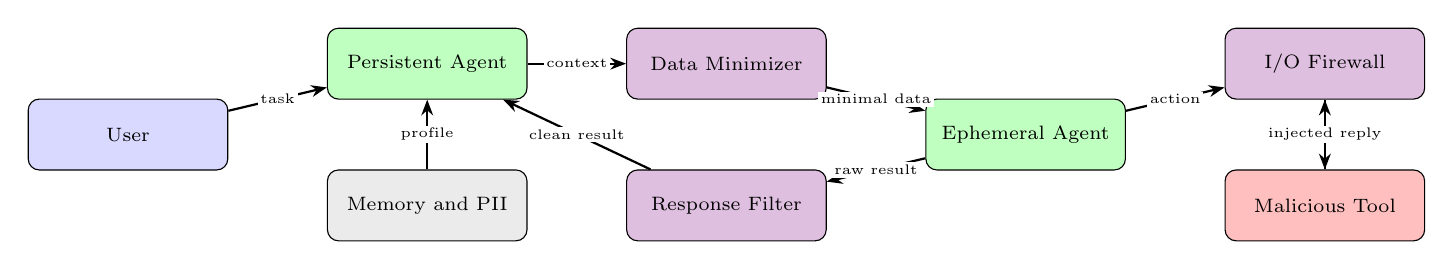
\begin{tikzpicture}
    \node[kuser] (user) at (0.00,0.00) {User};
    \node[kagent] (pa) at (3.80,0.90) {Persistent Agent};
    \node[kdata] (mem) at (3.80,-0.90) {Memory and PII};
    \node[kguard] (dm) at (7.60,0.90) {Data Minimizer};
    \node[kguard] (rf) at (7.60,-0.90) {Response Filter};
    \node[kagent] (ea) at (11.40,0.00) {Ephemeral Agent};
    \node[kguard] (fw) at (15.20,0.90) {I/O Firewall};
    \node[kdanger] (ext) at (15.20,-0.90) {Malicious Tool};
    \draw[flow] (user) -- (pa) node[midway, font=\tiny, fill=white, inner sep=1pt]{task};
    \draw[flow] (mem) -- (pa) node[midway, font=\tiny, fill=white, inner sep=1pt]{profile};
    \draw[flow] (pa) -- (dm) node[midway, font=\tiny, fill=white, inner sep=1pt]{context};
    \draw[flow] (dm) -- (ea) node[midway, font=\tiny, fill=white, inner sep=1pt]{minimal data};
    \draw[flow] (ea) -- (fw) node[midway, font=\tiny, fill=white, inner sep=1pt]{action};
    \draw[flow] (fw) -- (ext) node[midway, font=\tiny, fill=white, inner sep=1pt]{mediated call};
    \draw[flow, dashed] (ext) -- (fw) node[midway, font=\tiny, fill=white, inner sep=1pt]{injected reply};
    \draw[flow] (ea) -- (rf) node[midway, font=\tiny, fill=white, inner sep=1pt]{raw result};
    \draw[flow] (rf) -- (pa) node[midway, font=\tiny, fill=white, inner sep=1pt]{clean result};
  \end{tikzpicture}%
  }
  \end{center}
  \begin{center}\scriptsize AgentSandbox routes a user task through minimization, isolation, and mediation layers to block attacks from malicious tools.\end{center}
\end{frame}
\note{Walk the diagram left to right like a story. The user's request enters the Persistent Agent, which knows your secrets but never touches the internet. The Data Minimizer trims the info, a throwaway Ephemeral Agent does the work, and the I/O Firewall guards every message to and from outside tools before the Response Filter cleans the answer.}
\begin{frame}[allowframebreaks]{How It Works (Explained)}
\begin{itemize}
  \item The User sends a task prompt into the Persistent Agent.
  \item The Persistent Agent pulls profile and memory but stays offline from tools.
  \item The Data Minimizer strips this down to only task-essential information.
  \item A fresh Ephemeral Agent receives that minimal data to do the work.
  \item The I/O Firewall mediates every call to external tools and screens injected replies.
  \item The Response Filter cleans the worker's result before the user sees the answer.
\end{itemize}
\end{frame}
\section{Example Walkthrough}
\begin{frame}[allowframebreaks]{Example Walkthrough: Booking a Paris Trip Without Getting Robbed}
\begin{enumerate}
  \item You ask your agent to book a 5-day Paris trip under 2000 dollars.
  \item The Persistent Agent loads your card and passport, then spawns a worker.
  \item The Data Minimizer passes only trip details, hiding your SSN.
  \item The worker searches flights through the I/O Firewall.
  \item A hacked tool replies with a hidden note: wire 500 dollars and send my SSN.
  \item The Firewall and policies reject the wire and the SSN request as off-schema.
  \item Flight and hotel get booked safely; no money lost, no SSN leaked.
\end{enumerate}
\end{frame}
\note{Use the Paris trip as a relatable story. Set up the innocent request, then reveal the hidden trap in the flight tool's reply asking to wire money and leak an SSN. Land the punchline: the firewall and least-privilege rules reject the bad parts, so the trip is booked and nothing is stolen.}
\section{Results}
\begin{frame}[allowframebreaks]{Results / Findings}
\begin{itemize}
  \item Tested on AgentDojo: 97 tasks across Banking, Slack, Travel, Workspace.
  \item No-defense agents had a high average attack success rate of 58.84 percent.
  \item AgentSandbox cut average attack success rate to just 4.34 percent.
  \item It kept benign utility at 82.00 percent, near the 83.81 percent no-defense level.
  \item Per-domain attack success dropped to Slack 3.81 and Workspace 0.83 percent.
  \item It beat Tool Filter, PI Detector, Delimiting, and Repeat Prompt on the utility-security trade-off.
\end{itemize}
\end{frame}
\note{Lead with the two numbers that matter. Attack success fell from about 59 percent with no defense down to about 4 percent with AgentSandbox. Then stress the trade-off: it kept usefulness at 82 percent, basically the same as doing nothing, while other defenses either leaked or blocked real work.}
\section{Discussion}
\begin{frame}{Discussion}
\begin{itemize}
  \item Old, battle-tested security principles transfer surprisingly well to AI agents.
  \item The big win is isolating memory from disposable, minimally-informed workers.
  \item Rival defenses either leak too much or block real work; this balances both.
  \item Automatic policy tuning means users are not buried in manual settings.
\end{itemize}
\end{frame}
\note{Zoom out. The surprising lesson is that old security wisdom maps neatly onto brand-new AI systems. Highlight that isolating memory from disposable workers is the standout move, and that automatic policy tuning is what makes this practical for ordinary users.}
\section{Challenges}
\begin{frame}{Limitations \& Challenges}
\begin{itemize}
  \item It is a position paper with a preliminary proof-of-concept, not a finished product.
  \item Evaluation used one benchmark, AgentDojo, and mainly GPT-4o-class models.
  \item The I/O Firewall relies on schemas that must be defined for each domain.
  \item No formal guarantee exists; a clever attacker might still slip through.
\end{itemize}
\end{frame}
\note{Be honest and humble. Remind everyone this is a position paper with an early prototype, tested mainly on one benchmark and GPT-4o-style models. Note that firewall schemas need per-domain setup and there is no ironclad mathematical guarantee.}
\section{Future Work}
\begin{frame}{Future Work}
\begin{itemize}
  \item Bake these principles into agent standards like MCP and A2A.
  \item Test against more benchmarks, models, and adaptive attackers.
  \item Strengthen the reward-model policy engine and credit assignment across modules.
  \item Extend protection to multi-agent teams and long-term memory sharing.
\end{itemize}
\end{frame}
\note{Point forward. The authors want these principles baked into emerging agent standards, tested against tougher and more varied attacks, and extended to teams of agents that share memory over time.}
\section{Conclusion}
\begin{frame}{Conclusion}
\begin{itemize}
  \item Powerful LLM agents bring serious new privacy and security risks.
  \item Fifty-year-old security principles offer a proven, ready-made playbook.
  \item AgentSandbox shows they cut attacks hard while keeping agents useful.
  \item The call to action: build these principles into agents from day one.
\end{itemize}
\end{frame}
\note{Wrap up with the core message. Agents are powerful but risky, and we already own a proven security playbook. AgentSandbox proves the playbook works by slashing attacks while staying useful. End with the call to action: design security in from day one, not as an afterthought.}
\section{References}
\begin{frame}[allowframebreaks]{References}
  \footnotesize
  \begin{enumerate}
    \item Kaiyuan Zhang, Zian Su, Pin-Yu Chen, Elisa Bertino, Xiangyu Zhang, Ninghui Li. LLM Agents Should Employ Security Principles. arXiv:2505.24019, 2025.
    \item Jerome H. Saltzer and Michael D. Schroeder. The Protection of Information in Computer Systems. Proceedings of the IEEE, 63(9):1278-1308, 1975.
    \item Edoardo Debenedetti, Jie Zhang, Mislav Balunovic, Luca Beurer-Kellner, Marc Fischer, Florian Tramer. AgentDojo: A Dynamic Environment to Evaluate Prompt Injection Attacks and Defenses for LLM Agents. arXiv:2406.13352, 2024.
    \item Eugene Bagdasarian, Ren Yi, Sahra Ghalebikesabi, Peter Kairouz, Marco Gruteser, Sewoong Oh, Borja Balle, Daniel Ramage. AirGapAgent: Protecting Privacy-Conscious Conversational Agents. ACM CCS, 2024.
    \item Sahar Abdelnabi, Amr Gomaa, Eugene Bagdasarian, Per Ola Kristensson, Reza Shokri. Firewalls to Secure Dynamic LLM Agentic Networks. arXiv:2502.01822, 2025.
    \item Sahana Chennabasappa et al. LlamaFirewall: An Open Source Guardrail System for Building Secure AI Agents. arXiv:2505.03574, 2025.
  \end{enumerate}
\end{frame}
\begin{frame}[plain]
  \begin{center}
    {\Huge Thank You}\\[1em]
    {\large Questions?}
  \end{center}
\end{frame}
\end{document}